\documentclass{article}
\usepackage{wrapfig}
\usepackage{graphicx}
\usepackage{color}
\usepackage{enumitem,lipsum}
\usepackage[labelformat=empty]{caption}

\linespread{1.05}
\title{The Superhero Machine Learning Api}
\date{}
\begin{document}
    \maketitle
    % \thispagestyle{empty}
    Here at e-conomic we really love superheros. In fact we love superheros
    so much that we have decided to start a new department which will focus
    solely on inventing new superhero characters. Our team of dedicated
    inventors will think out new awesome characters and for each new creation
    the inventor will devise a character description containing information
    such as abilities, partnerships, team affiliations, etc.

    The two legendary US publishers, Marvel Comics and DC Comics, have shown
    great interest in our new department, and they would like to make offers
    on each new character.

    \begin{figure}[h]
        \minipage{0.5\textwidth}
            \centering
            
\includegraphics[width=0.7\textwidth]{marvel}
            \caption*{\scriptsize{Superheros published by Marvel Comics}}
        \endminipage\hfill
        \minipage{0.5\textwidth}
            \centering
            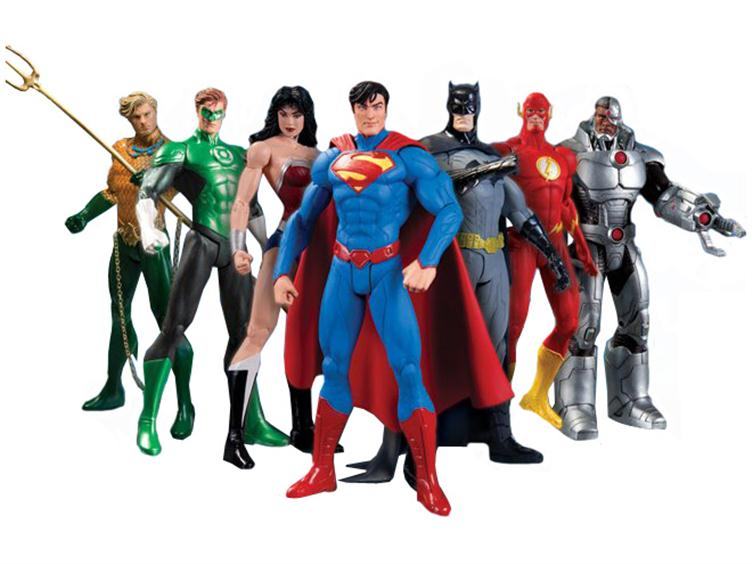
\includegraphics[width=0.8\textwidth]{dc}
            \caption*{\scriptsize{Superheros published by DC Comics}}
        \endminipage
    \end{figure}

    Due to market circumstances, when a new character is offered to a
    publisher, all other publishers lose interest in buying that character,
    because they are afraid that the company who got the offer first, may
    steal the idea and bring onto the market a similar superhero, before the
    investment can be legally secured.

    That is why we need your help! We mined Wikipedia for Marvel- and
    DC-superhero articles, and now we hand you the dataset\footnote{In the
    handout you will find \texttt{data.zip}}.

    Your task is to build a RESTful API that (\textit{i}) manages the
    articles, (\textit{ii}) and offers a prediction endpoint, that uses
    machine learning to classify a text as being either closer to the Marvel
    or the DC universe.

    \clearpage
    The API should use some kind of database for persistence and offer the
    following endpoints.
    \vspace{0.5cm}
    \begin{description}[labelindent=0.5cm, leftmargin=1cm]
        \item[\texttt{/article/(\$id)}] \hfill \\ 
            Article resource endpoint(s). The api should as minimum be able
            to read a resource, creates a resource, updates a resource,
            delete a resource and list resource URI's. The training data from
            \texttt{data.zip} should be posted to this endpoint.
        \item[\texttt{/train}] \hfill \\
            Train or re-train your machine learning model based on the
            articles in the database.
        \item[\texttt{/predict}] \hfill \\ 
            Receive a text as input and return classification results.
    \end{description} 
    \vspace{0.5cm}
    \noindent You will present the solution to a team of e-conomic developers
    and they might have questions and suggestions about the code and machine
    learning techniques. Keep in mind that we do not expect your code to be
    production ready. What we're looking for is how you approach the problem,
    preferably creating some nice and clean code along the way. We will
    appreciate if your solution is working and comes with a build guide, so
    that we can run and test it.

    When presenting the solution you are welcome to bring your own laptop if
    that suits you better. In case you have questions, please do not hesitate
    to ask.
    \\\\
    Happy coding :)
\end{document}
